\documentclass[final,a4paper,reqno]{elsarticle}
\setlength{
\textwidth}{5.9in}
\setlength{\oddsidemargin}{0.2in}
\setlength{\evensidemargin}{0.2in}
\setlength{\textheight}{8.75in}
\setlength{\topmargin}{0pt}
\setlength{\parindent}{15pt}
\setlength{\parskip}{5pt}

\usepackage{amssymb,amsmath,times,bbm,epsfig,float,fancyhdr}
%\usepackage[pdftex,pdftitle={Optimal control of reaction-diffusion equations},
%colorlinks=false,pdfstartview=FitH,breaklinks=true,linkcolor=blue]{hyperref}
\usepackage{amsmath}
\usepackage{wrapfig}
\usepackage{subfigure}
%\usepackage{slashbox}
\usepackage{xcolor}
\usepackage{tikz}

\newcommand{\cblue}[1]{\textcolor{blue}{#1}}

\graphicspath{{figures/}}

\usepackage{algorithm2e}
%\usepackage{algorithmic}
\usepackage{refcheck}
\numberwithin{equation}{section}
\newcommand{\fracd}[2]{\displaystyle {\frac{{\displaystyle{#1}}}{{\displaystyle{#2}}}}}
\newcommand{\diag}{\operatorname*{diag}}
\renewcommand{\aa}{\ensuremath{\mathbf{a}}}
\newcommand{\norm}[1]{\ensuremath{\left\|#1\right\|}}
\newcommand{\abs}[1]{\ensuremath{\left|#1\right|}}
\newcommand{\bu}{\ensuremath{\mathbf{u}}}
\newcommand{\Div}{\nabla\cdot\,}
\newcommand{\oDiv}{\overline{\nabla}\cdot\,}
\newcommand{\ee}{\ensuremath{\mathbf{e}}}
\newcommand{\eps}{\ensuremath{\varepsilon}}

\newcommand\escala{\tilde{\varphi}}
\newcommand{\G}{\ensuremath{\mathcal{G}}}
\newcommand{\mP}{\ensuremath{\mathcal{P}}}
\newcommand{\Grad}{\ensuremath{\mathrm{\nabla}}}
\newcommand{\oGrad}{\ensuremath{\mathrm{\overline{\nabla}}}}
\renewcommand{\k}{\ensuremath{\mathbf{k}}}
\newcommand{\M}{\ensuremath{\mathcal{M}}}
\newcommand{\N}{\ensuremath{\mathbb{N}}}
\newcommand{\n}{\ensuremath{\mathbf{n}}}


%\newcommand{\sgn}{\mathrm{sign}}



\newcommand{\bMe}{\ensuremath{\mathbf{M}_{\mathrm{e}}}}
\newcommand{\bMi}{\ensuremath{\mathbf{M}_{\mathrm{i}}}}
\newcommand{\bMs}{\ensuremath{\mathbf{M}_{\mathrm{s}}}}
\newcommand{\bMj}{\ensuremath{\mathbf{M}_{\mathrm{j}}}}

\newcommand{\bC}{\ensuremath{\mathbf{C}}}
\newcommand{\Iona}{I_{1,\mathrm{ion}}}
\newcommand{\tIona}{\tilde{I}_{1,\mathrm{ion}}}
\newcommand{\Ionb}{I_{2,\mathrm{ion}}}
\newcommand{\sn}{\sum_{n=0}^{N-1}}
\newcommand{\A}{\ensuremath{\mathcal{A}}}

\def\dist{{\rm dist\,}}
\def\meas{{\rm meas\,}}

\def\bzeros{\mathbf{0}}
\def\bL{\mathbf{L}}
\def\bH{\mathbf{H}}
\def\bP{\mathbf{P}}
\def\bV{\mathbf{V}}

\newcommand{\seq}[1]{\left<#1\right>}
\newcommand{\Real}{\mathbb R}
\newcommand{\Natural}{\mathbb N}
\newcommand{\Complex}{\mathbb C}
\newcommand{\Field}{\mathbb F}
\newcommand{\RPlus}{[0,\infty)}
\newcommand{\Lagrangian}{\mathcal{L}}
\newcommand{\Phat}{(\hat{\textrm{P}})}
\def\Ai {{\mathbf{A_i}}}
\def\Aie {{\mathbf{A_{ie}}}}
\def\M {{\mathbf{M}}}

\def\B {{\mathbf{B}}}

\def\Mtilde {\tilde{\mathbf{M}}}
\def\F {{\mathbf{F}}}
\def\G {{\mathbf{G}}}
\def\b {{\mathbf{b}}}
\def\u {{\mathbf{u}}}
\def\v {{\mathbf{v}}}
\def\V {{\mathbf{V}}}
\def\W {{\mathbf{W}}}
\def\p {{\mathbf{p}}}
\def\q {{\mathbf{q}}}
\def\c {{\mathbf{c}}}
\def\VK{V^{K}_h}
\def\HdoK{{H^{2}(K)}}

%%%%%%%%%%%%%%%%%%%%
\newcommand{\T}{\mathcal{T}}
\newcommand{\Vh}{\boldsymbol{\mathcal{V}}^h}
\newcommand{\bv}{\boldsymbol{v}}
\newcommand{\bw}{\boldsymbol{w}}
\newcommand{\bp}{\boldsymbol{p}}
\newcommand{\br}{\boldsymbol{r}}
\newcommand{\bpi}{\boldsymbol{\Pi}}
\newcommand{\si}{\sum_{i=1}^N}
\newcommand{\sij}{\sum_{i,j=1}^N}
\newcommand{\I}{\mathcal{I}}

%%%%%%%%%%%%%%%%%
%%%%%%%%%%%%%%%%%%
\newcommand{\charu}{{1\hspace*{-3.5pt}1}}
%\def\I{{\!|\!}}
\def\ptI{{\!,}}
\def\ptK{{K}}
\def\ptL{{L}}
\def\K{{K}}
\def\L{{L}}
\def\xK{{x_\ptK}}
\def\xL{{x_\ptL}}
\def\KL{{\K\!,\!\L}}
\def\ptKL{{\ptK,\ptL}}
\def\ptptl{{\ptl}}
\def\KIL{{{\textstyle\sigma}_{\!\!\K,\!\L}}}
\def\ptKL{{\ptK,\ptL}}
\def\ptKIL{{\!\ptK\ptI\ptL}}
\def\mKIL{{|{\textstyle\sigma}_\ptKIL|}}  % {{|{\textstyle\sigma}_{{\!{{K}}{{\!,}}{{L}}}}|}}
\def\mK{{|K|}}
\def\dKL{{d_{\ptK,\ptL}}}
\def\nuKL{{\eta_{\ptK,\ptL}}}
\def\Del{{\scriptstyle \Delta}}
\def\diam{{\rm diam\,}}


%%%%%%%%%%%%%%%%%%
\newcommand{\R}{{\mathbb R}}
\def\Drond{{\boldsymbol{\mathfrak D}}}
\def\Mrond{{\boldsymbol{\mathfrak M}^{\hspace*{-1pt}o}}}
\def\Tau{{\boldsymbol{\mathfrak T}}}
\def\DM{{\scriptstyle D}}
\def\ptD{{\scriptscriptstyle D}}
\def\dMrond{{\boldsymbol{\mathfrak M}}}
\def\xdKi{{x_{\ptK_{\!i}}}}
\def\dK{{\scriptstyle K}}
\def\ptl{{\partial}}
\def\xdK{{x_\ptdK}}
\def\ptdK{{\scriptscriptstyle K}}
\def\ptK{{\scriptscriptstyle K}}
\def\SDM{{\scriptstyle S}}
\def\dVrond{{{\scriptstyle\mathcal V}}}
\def\Srond{{\boldsymbol{\mathfrak S}}}
\def\ptS{{\scriptscriptstyle S}}
\def\K{{\scriptstyle K}}
\def\epsSdK{{\epsilon_\ptS^\ptdK}}
\def\ptTau{{\scriptscriptstyle \boldsymbol{\mathfrak T}}}
\def\wdK{{w_\ptdK}}
\def\ptdMrond{{\scriptscriptstyle \boldsymbol{\mathfrak M}}}
\def\char{{1\!\mbox{\rm l}}}
\def\ptbarTau{{\overline{\ptTau}}}
\def\ptBleft{{\Bigl[\hspace*{-3pt}\Bigl[}}
\def\ptBright{{\Bigr]\hspace*{-3pt}\Bigr]}}
\def\Vol{{\text{\footnotesize \sl Vol}}}
\def\Frond{{\mathcal M}}
\def\ptDrond{{\scriptscriptstyle \boldsymbol{\mathfrak D}}}
\def\ptAleft{{\Bigl\{\!\!\!\Bigl\{}}
\def\Grond{{\mathcal G}}
\def\ptAright{{\Bigr\}\!\!\!\Bigr\}}}
\def\grad{{\,\nabla }}
\def\ProjD{{\text{Proj}_\ptD}}
\def\dsp{\displaystyle}
\def\ptdVrond{{{\scriptscriptstyle\mathcal V}}}
\def\ptepsSdK{{ \textstyle\epsilon_{\scriptscriptstyle S}^{ \scriptscriptstyle K} }}
\newcommand{\divi}{{\rm div \,}}
\def\edgeS{{\edge_\ptS}}
\def\Bleft{{\bigl[\hspace*{-3pt}\bigl[}}
\def\Bright{{\bigr]\hspace*{-3pt}\bigr]}}
\def\Aleft{{\biggl\{\!\!\!\biggl\{}}
\def\Aright{{\biggr\}\!\!\!\biggr\}}}
\def\Cleft{{\biggl<\hspace*{-4pt}\biggl<}}
\def\Cright{{\biggr>\hspace*{-4pt}\biggr>}}
\def\edge{{\sigma}}
\def\ptdelt{{ {\scriptscriptstyle \Delta}t }}
\def\Ndelt{{ N_{\!\ptdelt} }}
\def\size{{\text{size}}}
\def\Delt{{{\scriptstyle \Delta} t}}
\def\ptDelt{{{\scriptscriptstyle \Delta} \scriptstyle t}}
\def\delt{{ {\scriptstyle \Delta}t }}
\def\ph{{\varphi}}
\def\D{{D}}
\def\xidemi{{x_{\hspace*{-1pt}i\hspace*{-1pt},
\hspace*{-1pt}i\hspace*{-1pt}{\scriptscriptstyle +}\!{\scriptscriptstyle 1}}}}


%%%%%%%%%%%%%
\newcommand{\bsig}{\boldsymbol{\sigma}}
\newcommand{\btau}{\boldsymbol{\tau}}
\newcommand{\bvarphi}{\boldsymbol{\varphi}}
\newcommand{\bx}{\ensuremath{\boldsymbol{x}}}
\newcommand{\bD}{\ensuremath{\mathbf{D}}}
\newcommand{\bpsi}{\boldsymbol{\psi}}
\newcommand{\ff}{\boldsymbol{f}}

%%%%%%%%%%%%%%


\newcommand{\Om}{\ensuremath{\Omega}}
\newcommand{\pt}{\ensuremath{\partial_t}}
\newcommand{\pxi}{\ensuremath{\partial_{x_i}}}
\renewcommand{\r}{\ensuremath{\mathbf{r}}}
\newcommand{\RR}{\mathbb{R}}
\newcommand{\w}{\ensuremath{\mathbf{w}}}
\newcommand\wavelet{\tilde{\psi}}
\newcommand{\x}{\ensuremath{\mathbf{x}}}
\newcommand{\sgn}{\mathrm{sign}}
\newcommand{\op}{\ensuremath{\overline{p}}}
\newcommand{\oq}{\ensuremath{\overline{q}}}
\newcommand{\opi}{\ensuremath{\overline{p}_i}}
\newcommand{\ops}{\ensuremath{\op^\star}}
\renewcommand{\u}{\mathbf{u}}
\newcommand{\ue}{\ensuremath{u_\eps}}
\newcommand{\uei}{\ensuremath{u_{i,\eps}}}
\newcommand{\Iap}{I_{\mathrm{app}}}
\newcommand{\Ion}{I_{\mathrm{ion}}}
\newcommand{\Iaph}{I_{\mathrm{app},h}}
\newcommand{\IapK}{I_{\mathrm{app},K}}
\newcommand{\Iape}{I_{\mathrm{app},\eps}}
\newcommand{\Iapn}{I_{\mathrm{app},n}}
\newcommand{\IonK}{I_{\mathrm{ion},K}}
\newcommand{\Iapnk}{I_{\mathrm{app},n}^\kappa}
\newcommand{\dx}{\ensuremath{\, dx}}
\newcommand{\dy}{\ensuremath{\, dy}}
\newcommand{\dz}{\ensuremath{\, dz}}
\newcommand{\dt}{\ensuremath{\, dt}}
\newcommand{\ds}{\ensuremath{\, ds}}
\newcommand{\dr}{\ensuremath{\, dr}}
\def\e{{\text{e}}}
\newcommand{\EE}{\mathcal{E}}
\newcommand{\TT}{\mathcal{T}}
\newcommand{\bA}{\mathbf{A}}
\newcommand{\bM}{\ensuremath{\mathbf{M}}}
%\newcommand{\I}{\mathcal{I}}

\newcommand{\tH}{\ensuremath{\tilde{H}^1(\Omega_H)}}

\newtheorem{alg}{Algorithm}%[section]
\newtheorem{thm}{Theorem}[section]
\newtheorem{rem}{Remark}[section]
\newtheorem{lem}[thm]{Lemma}
\newtheorem{defi}{Definition}[section]
\newtheorem{prop}{Proposition}[section]
%\newproof{proof}[thm]{Proof}
\newenvironment{proof}[1][Proof]{\noindent\textit{#1.} }{\hfill \rule{0.5em}{0.5em}}
\allowdisplaybreaks
%\pagestyle{fancy}
%\lhead{\em Optimal control for electrical heart activity}

% track changes and comments
%\usepackage[textsize=scriptsize]{todonotes}
%\usepackage[final]{changes}
%\definechangesauthor[color=green]{GR}
%\setremarkmarkup{\todo[color=Changes@Color#1!40]{\textcolor{black}{#1:{#2}}}}
%\setauthormarkupposition{left}
%\newcommand\redout{\bgroup\markoverwith{\textcolor{red}{\rule[.5ex]{2pt}{0.4pt}}}\ULon}
%\setdeletedmarkup{\redout{#1}}
%\newcommand{\comment}[1]{\todo[color=Changes@ColorGR!40]{\color{black}Note: #1}}
%\newcommand{\todocite}[1]{[?\todo[color=red]{TODO cite: {#1}}]}

\begin{document}

\begin{frontmatter}
%************************************************
\title{ An adaptive nonlinear SIR  epidemic model for  CoviD-19 disease spreading  and forecasting }

\author[2]{ Said Gounane  }
\ead{...}
\author[2]{Yassir Barkouch }
\ead{...}
\author[3]{Abdelghafour Atlas }
\ead{a.atlas@uca.ma}
%
\author[1]{Mostafa Bendahmane}
\ead{mostafa.bendahmane@u-bordeaux.fr}

\author[2]{Fahd Karami}
\ead{fa.karami@uca.ma}

%
\address[1]{Institut de math\'ematique de Bordeaux (IMB) et l'institue de rythmologie et mod\'elisation cardiaque (Liryc), universit\'e de Bordeaux et INRIA-Carmen Bordeaux Sud-Ouest}
\address[2]{Ecole Supérieure de Technologie d'Essaouira Km 9, Route d'Agadir, Essaouira Aljadida BP. 383, Essaouira. Maroc.}
\address[3]{Ecole Nationale des sciences appliqu\'ess ....Marrakech. Maroc.}


\begin{abstract}
A various  mathematical models of the COVID-19 coronavirus has been proposed. We develop here a model describing this epidemic,
focused on the  impact of moroccan government imposed public policies designed to contain this
epidemic. The proposed model  is a general form  SIR and SIER epidemic in \cite{KeMc}. We identify a constant transmission rate ...

\textit{ Recently, a various mathematical models has been proposed and used for modeling and forecasting COVID-19 disease. But, all of this forecasting results have been interpreted and computed with fixed data (based on governmental data sources)  until a specified day and time and there are not taking account of the recent changed data and the evolution  of the pandemie situation. The first aims of this platform is develop an interactive application wich is  able to simulate and forecasting the spread of Covid-19, based on the classical models likes SIR, SEIR and their variants at each time with the actual update of real data that  come from different API. The Simulator-Covid  page allow to simulate the presented mathematical models for a various values of the model parameter?s. To find the parameters adopted for each countries ( in particular in morocco and its regions ) and we fit the models for each country with respect to the actual real data given by the API . The second aims is to present  some recents models (developed by our team) describes the spreading of coronavirus under the effect of a various government measures related to stoping coronavirus spreading, likes lockdowns or confinement. We also evaluate the  government measures a each country and  investigate the clustering of  country with respect to the evolution of the pandemic. }
\end{abstract}

\begin{keyword} ...\sep ...
%\MSC 74S05 \sep 65M99 \sep 35K65
\end{keyword}
\date{\today}
\end{frontmatter}
\section{Introduction}\label{sec:intro}
%%%%%%%%%%%%%%%%%%%%%%
The worldwide spread of the new  coronavirus that causes severe acute  respiratory  syndrome   has  led more than 180  countries. 
This virus has affected more than  5 million and caused the death of  350.000 people  at 20th May and which also affects the world economy.  The World Health Organization (WHO) named the pneumonia caused by the new coronavirus COVID-19. The International Committee on Taxonomy of Viruses named it  SARS-CoV-2.  SARS-CoV-2 is a coronavirus similar to SARS-CoV and MERS-CoV. SARS-CoV first occurred from November 2002 to June 2003 in Guangdong, China, and spread to many parts of the world. MERS-CoV was found in 2012 in Saudi Arabia. In the fight against this virus and the absence of a treating vaccine, the international community has more interest in putting in place tools which illustrate the principle of its virality and which aim to understand and consequently to control the spread of the virus and / or to mitigate it. This global health crisis of Covid-19 has brought to light the primordial role of the development of research and scientific evolution. In particular, the role of mathematical modeling in understanding the spread of the disease over time.  In front of this situation of invasion of covid19 on an international scale, access is now facilitated to much more data and even to analyzes carried out by scientists and researchers around the world. However, modeling and forecasting the spread of COVID-19 remains an urgent challenge to draw up data based on data in other countries over the long term. In our project, we present a basic models of epidemic transmission that can be linked to data provided by international scientific reports and to data from different cities in Morocco. \\
%%%%%%%%%%%%%%%%%%%%%%

When no vaccine is available, the isolation of diagnosed infectives and social distancing are the only control measures available.\\
%


%%%%%%%%%%%%%%%%%%%%%%
\section{Mathematical model }

%%%%%%%%%%%%%%%
\subsection{ The SIR  model }\label{sir}

\noindent The SIR model is one of the most epidemiological compartmental
models for  the investigation of the spread of disease caused by virus. This model  was introduced by Kermack
and McKendrick in $1927$ to describes the evolution of the relative proportions of three  disjoint  classes  which change with time $t$  

\begin{figure}[!h]
\centering
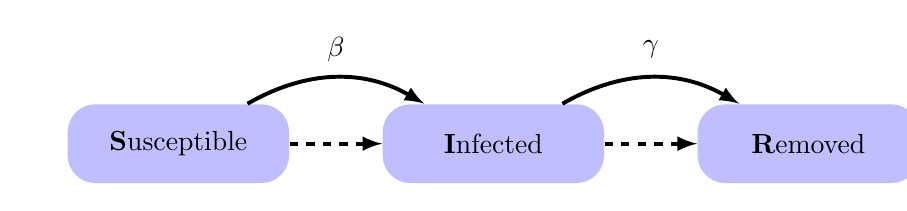
\begin{tikzpicture}
\tikzstyle{point}=[rectangle, rounded corners=10pt,fill=blue!25,minimum width=8em, minimum height=1cm]
\tikzstyle{fleche}=[->,>=latex,line width=0.5mm]
\node[point] (N) at (4,0){\textbf{S}usceptible};
\node[point] (S) at (8,0){\textbf{I}nfected };
\node[point] (R) at (12,0){\textbf{R}emoved };
\draw[fleche] (N) edge [bend left] (S)  ;
\draw[fleche] (N) edge[dashed] (S)  ;
\draw[fleche] (S) edge [bend left](R);
\draw[fleche] (S) edge[dashed] (R)  ;
\draw (6,1.2) node {$\bf{\beta}$} ;
\draw (10,1.2) node {$\bf{\gamma}$} ;
\end{tikzpicture}
\caption{ Compartemental diagram for SIR model};
\end{figure}

\noindent In the SIR model, the population
is subdivided into the following three epidemiologically distinct types of individuals and  this classes are be represented by
\begin{enumerate}
\item   The susceptible class $\textbf{S}(t)$  the individuals  have not yet  infected by
the disease of interest . 
\item  The infected class $\textbf{I}(t)$ the individuals who
are currently infected and capable to transmitting the disease to others. 
\item The removed class $\textbf{R}(t)$ the individuals  formally infected
who are deceased, or have recovered and are either permanently immune.
\end{enumerate}
Mathematically, the model can formulated as a system of three equations  \cite{KeMc}:
\begin{equation}\label{Sir-system}
\begin{cases}
\displaystyle \frac{ dS(t)}{dt} = -\frac{\beta}{N} S(t) \: I(t)\\ \\
\displaystyle  \frac{ dI(t)}{dt}  = \frac{\beta}{N} S(t) \: I(t) -\gamma I(t)\\  \\
\displaystyle  \frac{ dR(t)}{dt} = \gamma I(t). 
\end{cases}
\end{equation}
 The term $\frac{\beta}{N} S(t) \: I(t)$ represents the disease transmission rate by contact between susceptible and infected individuals.  The parameter  $\beta$ is the infection rate (to be estimated) and $\gamma$ is the recovery rate which can be computed with respect to the period of viral shedding ( $\gamma\sim \frac{1}{10} days^{-1}$ in the case of Covid-19). Adding all equations in the model, we observe that  the total population  $N=S+I+R$ is a constant. Indeed, we see that   
$$ \displaystyle \frac{ dS(t)}{dt} +   \frac{ dI(t)}{dt}  +  \frac{ dR(t)}{dt} = 0 \qquad \mbox{ and }\;\;  S(t)+I(t)+R(t)=N \mbox{ for each time  } t.$$ 
The system (\ref{Sir-system}) are completed by the initial conditions. Starting the model when the first infected
individual appears in the population, which  correspond to 
$ \displaystyle S(0)=N,  \: I(0)=0$ and  $R(0)=0$. The case where the number  of infected and recovered is neglected with respect to the total population the number of susceptible $S$ in can be approximated by a constant, $ S(t) \sim S(0)=N$. The first  equation (\ref{Sir-system}) can be written as 
  \begin{equation}\label{Sir-simplified}
\displaystyle  \frac{ dI(t)}{dt}  \sim \beta \: I(t) -\gamma I(t).
\end{equation}
We obtain an ordinary differential equation with constant coefficients and the solution can be expressed as
\begin{equation}\label{Sir-sol}
\displaystyle  I(t)  \sim I(0) \: \exp((\beta-\gamma)t)
\end{equation}
Based on available data, this exponential growth is observed in the first days of  starting COVID-19 outbreak data from various countries.
%with remarkably similar estimated %doubling times in the early stages of the epidemic.
\subsection{ The SIRD  model }
Now, let us consider the SIR model (\ref{Sir-system}) with additional class $D(t)$ of deaths individuals  due to the epidemic and $\sigma$ the mortality rate of the infected.  
We will note by $\textbf{R}(t)$  the recovered class and model can be expressed by
\begin{figure}[!h]
\centering
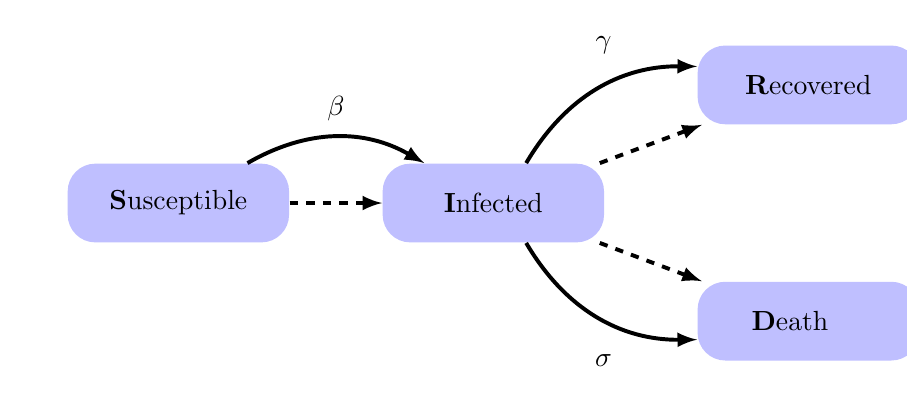
\begin{tikzpicture}
\tikzstyle{point}=[rectangle, rounded corners=10pt,fill=blue!25,minimum width=8em, minimum height=1cm]
\tikzstyle{fleche}=[->,>=latex,line width=0.5mm]
\node[point] (N) at (4,0){\textbf{S}usceptible};
\node[point] (S) at (8,0){\textbf{I}nfected };
\node[point] (R) at (12,1.5){\textbf{R}ecovered };
\node[point] (D) at (12,-1.5){ \quad \textbf{D}eath \qquad \qquad };
\draw[fleche] (N) edge [bend left] (S)  ;
\draw[fleche] (N) edge[dashed] (S)  ;
\draw[fleche] (S) edge [bend left](R);
\draw[fleche] (S) edge[dashed] (R)  ;
\draw[fleche] (S) edge [bend right](D);
\draw[fleche] (S) edge[dashed] (D)  ;
\draw (6,1.2) node {$\bf{\beta}$} ;
\draw (9.4,2) node {$\bf{\gamma}$} ;
\draw (9.4,-2) node {$\bf{\sigma}$} ;
\end{tikzpicture}
\caption{ Compartemental diagram for SIRD model};
\end{figure}

The dynamics of $D(t)$ depends on $I(t)$ and the SIRD System can be written as
\begin{equation}\label{SirD-system}
\begin{cases}
\displaystyle \frac{ dS(t)}{dt} = -\frac{\beta}{N} S(t) \: I(t)\\ \\
\displaystyle  \frac{ dI(t)}{dt}  = \frac{\beta}{N} S(t) \: I(t) -(\gamma+\sigma) I(t)\\  \\
\displaystyle  \frac{ dR(t)}{dt} = \gamma I(t) \\ \\
\displaystyle  \frac{ dD(t)}{dt} = \sigma I(t).
\end{cases}
\end{equation}
 Adding all equations in the model, we observe that  the total population  $N=S+I+R+D$ is a constant. Indeed, we see that   
$$ \displaystyle \frac{ dS(t)}{dt} +   \frac{ dI(t)}{dt}  +  \frac{ dR(t)}{dt}+\frac{ dD(t)}{dt} = 0 \qquad \mbox{ and }\;\;  S(t)+I(t)+R(t)+D(t)= N\mbox{ for each time  } t.$$
Now, thanks to  \cite{Mu},  the basic reproduction number of  (\ref{SirD-system}) can be computed by $$\mathcal{R}_0=  \frac{\beta S(0)}{ (\gamma+\sigma)N}.$$ 
Similarly as in subsection (\ref{sir} ),  we have $ \displaystyle  I(t)  \sim I(0) \: \exp((\beta-\gamma-\sigma)t)$ for $S(0)\sim N$. In this case,   we see that  the number of infected will grow for  $\beta>\gamma+\sigma$ i.e.  $\mathcal{R}_0>1$ and when  $\beta-\gamma -\sigma<0$ i.e.  $\mathcal{R}_0<1$ it will decay which plays the key role behind disease propagation. For more analysis about this  see, for instance\cite{We, Mu,DiHe}.

\subsection{ The proposed non linear SIRD  model }
In this work, we assume the human behavior to propagation of diseases and which individuals reduce their contacts with respect to the increasing  of affected  individuals, and we  propose a modified SIRD model with social distancing  which can expressed as 
\begin{equation}\label{Sir-gen-system}
\begin{cases}
\displaystyle \frac{ dS(t)}{dt} = -{\beta} \Big[\frac{S(t)}{N}\Big]^{p(t)} \: I(t)\\ \\
\displaystyle  \frac{ dI(t)}{dt}  = {\beta} \Big[\frac{S(t)}{N}\Big]^{p(t)}  I(t)\ -(\gamma+\sigma) I(t)\\  \\
\displaystyle  \frac{ dR(t)}{dt} = \gamma I(t) \\ \\
\displaystyle  \frac{ dD(t)}{dt} = \sigma I(t).
\end{cases}
\end{equation}
where $p(t)\geq 1$ is a continuous function  such that $p(0)=1$ and $p(t)\to p^\star$ as $t\to \infty $. The function $p(t)$ describe the social distancing  and the sensitivity to disease. For $p(t)=1$, we recover the SIRD model (\ref{SirD-system}). In  general, after the start of the evolution of the epidemic,
there is a  large reduction in the population $S(t)$ by a social distancing measures.  For that, we assume that
$ p(t)= 1$  for $ t\leq t_c$ and  $ p(t)= p^\star$  for $t\geq t_c$, where $t_c$ is the time of beginning confinement. A typical example is

\begin{equation}\label{p}
p_\varepsilon(t)=
\begin{cases}
\displaystyle 1  &\qquad \mbox{if}  \qquad  t\leq t_c\\ 
\displaystyle  \frac{p^\star-1}{\varepsilon} (t-t_c) + 1 & \qquad \mbox{if}  \qquad t_c \leq t\leq t_c+\varepsilon\\ 
\displaystyle  p^\star  &\qquad \mbox{if}  \qquad  t\geq t_c+\varepsilon
\end{cases}
\end{equation}


\subsubsection{The reproduction number and phase plane}
\noindent Observe that the non trivial equilibrium values of the system (\ref{Sir-gen-system}) is given by $(S^\star,0,R^\star,D^\star)$ where
 $$\displaystyle S^\star= N\Big(\frac{\gamma+\sigma}{\beta}\Big)^{\frac{1}{p^\star}} \quad \mbox{and }\;  R^\star+D^\star=N(1-\Big(\frac{\gamma+\sigma}{\beta}\Big)^{\frac{1}{p^\star}} ).$$ 
Recall that, the total population $S(t) + I(t) + R(t) +D(t)=N$  of each $t$, we focus only on the equation
in $S$ and $I$. Following \cite{DrWat, DiHe},  the right side of the  system (\ref{Sir-gen-system})  can be decomposed as 
$\displaystyle \mathcal{F}+\mathcal{V}^++\mathcal{V}^-$ where 
$$\displaystyle \mathcal{F}(S,I)= (0,{\beta} \Big[\frac{S}{N}\Big]^{p} I ), \quad \mathcal{V}^+(S,I)=(0,0) \quad \mbox{ and }\quad \mathcal{V}^-(S,I)=(-{\beta} \Big[\frac{S}{N}\Big]^{p} I,-(\gamma+\sigma) I ).$$
then, we have $\displaystyle F= {\beta} \Big[\frac{S^*}{N}\Big]^{p^*} $ and $V=-(\gamma+\sigma)$, we deduce that 
 $$\mathcal{R}_{0}= \rho(-FV^{-1})= \frac{\beta}{\gamma+\sigma} \Big[\frac{S}{N}\Big]^{p^*} .$$
 where $\rho$ is a spectral radius. Moreover, the number of people in a population who can be infected by an individual at time $t$ can be represented by  the effective reproduction number:   $$R^p_t= \frac{\beta}{\gamma+\sigma} \Big[\frac{S(t)}{N}\Big]^{p(t)}.$$ 
 We observe that the social distancing affect $R_t$, since $S(t)\leq N$ and when $p\to \infty$ we observe that $R^p_t \to 0.$


\noindent Now, we investigate the phase plane, dividing the first equation  by  the second in (\ref{Sir-gen-system}), the phase portrait
for the epidemic, can be formulated as 
\begin{equation}\label{IS}
\displaystyle \frac{ dI}{dS} = \frac{\gamma+\sigma}{ \beta } \Big[\frac{S}{N}\Big]^{-p(t)}  -1.\\ \\
\end{equation}
Integrating this equation with respect to $S$,  for any $t>t_c$ we have 
\begin{equation}
\begin{array}{ll}
 I (t) &= I(t_0) + \displaystyle   \frac{  N}{\mathcal{R}_0 }  \int^{t_c}_{t_0} \frac{  1}{ \:S} dS+  \frac{  1}{\mathcal{R}_0 } \lim_{\varepsilon \to 0}  \int^t_{t_c+\varepsilon} \Big[\frac{S}{N}\Big]^{-p(t)} dS- \int^{t}_{t_0}  dS \\ \\
 &\displaystyle =  I(t_0) +\frac{N}{\mathcal{R}_0} \ln\Big(\frac{S(t_c)}{S(t_0)}\Big)+\frac{ N}{\mathcal{R}_0 (1-p(t)) } \Big[\frac{S(t)}{N}\Big]^{1-p(t)}\\ \\
 & \displaystyle- \lim_{\varepsilon \to 0}  \frac{ N}{ \mathcal{R}_0 (1-p(t_c+\varepsilon)) } \Big[\frac{S(t_c+\varepsilon)}{N}\Big]^{1-p(t_c+\varepsilon)}+S(t_0)-S(t)\\ \\
 &\displaystyle =  I(t_0) +\frac{N}{\mathcal{R}_0} \ln\Big(\frac{N}{S(t_0)}  \Big) - \frac{ N}{\mathcal{R}_0 (1-p(t)) } \Big[\frac{S(t)}{N}\Big]^{1-p(t)}+S(t_0)-S(t)
\end{array}
\end{equation}
Since $$\displaystyle \frac{ d^2I}{dS^2}  =\frac{-p(t)}{ N \mathcal{R}_0  } \Big[\frac{S}{N}\Big]^{-p(t)-1} \leq 0,$$  we assume that the maximum $ I_{max}$ reach  after $t_c$ then  $I_{max}$ occurs when $\frac{ dI}{dt}=0$ or in the other words $\displaystyle S^\star= N \mathcal{R}_0^{\frac{1}{p^\star}} $ then we can compute the maximum number of infective
 $$ I_{max}=   I(t_0) +\frac{N}{\mathcal{R}_0} \ln\Big(\frac{N}{S(t_0)}  \Big) +\frac{ N}{ (1-p^*) } \Big[\mathcal{R}_0\Big]^{\frac{1}{p^*}-2}+S(t_0)-N \mathcal{R}_0^{\frac{1}{p^\star}}
$$
Starting the model when the first infected
individual appears in the population, which  correspond to 
$ \displaystyle S(t_0)=N$ and  $I(0)=0,$ then

 $$ I_{max}=   \frac{ N}{ (1-p^*) } \Big[\mathcal{R}_0\Big]^{\frac{1}{p^*}-2}+N(1- \mathcal{R}_0^{\frac{1}{p^\star}}).
$$

\subsection{ Numerical simulations}
\noindent Generally, explicit treatment of  (\ref{Sir-system}) usually means stricter conditions on time step and the parameters  to
achieve stability of time discretization schemes. To overcome this, we will use   the implicit Euler method, discretizing the time variable as $t = k \tau$ where $k$ is a number and $\tau$ is the time step.
The discrete iterative scheme of the proposed model  can be written as
\begin{equation}\label{Sir-system_d}
\begin{cases}
\displaystyle S_{k+1} = S_{k} -\tau {\beta}  \Big[\frac{S_{k+1}}{N}\Big]^{p_{k+1}}\: I_{k+1}\\ \\
\displaystyle  I_{k+1} = I_{k} +\tau {\beta}  \Big[\frac{S_{k+1}}{N}\Big]^{p_{k+1}} I_{k+1} -\tau (\gamma+\sigma) I_{k+1}\\ \\
\displaystyle  R_{k+1} = R_{k} +\tau  \gamma I_{k+1}  \\ \\
\displaystyle  D_{k+1} = D_{k} +\tau  \sigma I_{k+1}
\end{cases}
\end{equation}
where $S_{k+1}$, $I_{k+1}$, $R_{k+1}$  and  $R_{k+1}$ are number of  the susceptible,  the infected and the recovered and death in the specific day $k+1$ respectively, $p_{k+1}$ the value if $p$ at day $k+1$. First, assume that  $p_{k}=1$ for any $k\geq 0$, the discrete (\label{Sir-system_d}) iterative scheme becomes
\begin{equation}\label{Sir-system-di2}
\begin{cases}
\displaystyle S_{k+1} = S_{k} -\tau \frac{\beta}{N} \: S_{k+1}\: I_{k+1}\\ \\
\displaystyle  I_{k+1} = I_{k} +\tau \frac{\beta}{N}  \: S_{k+1} \: I_{k+1} -\tau( \gamma+\sigma) I_{k+1}\\ \\
\displaystyle  R_{k+1} = R_{k} +\tau  \gamma I_{k+1}  \\ \\
\displaystyle  D_{k+1} = D_{k} +\tau  \sigma I_{k+1}
\end{cases}
\end{equation}
 Adding the first and the second equations, we obtain 
\begin{equation}\label{Eq1}
\displaystyle(1+\tau (\gamma+\sigma)) I_{k+1} =  I_{k}+S_{k} - \: S_{k+1}. 
\end{equation}
From the first equation, we have 
\begin{equation}\label{Eq2}
\displaystyle S_{k+1} =  \frac{S_{k} }{1+\tau \frac{\beta}{N} I_{k+1}}. 
\end{equation}
Replacing (\ref{Eq2}) in  (\ref{Eq1}) and the fact that $S_{k} +I_{k}+R_{k}+D_{k}=N$, we can easily obtain that
\begin{equation}\label{Eq3}
\displaystyle I_{k+1} =  \frac{\sqrt{\Big(\tau( \gamma+\sigma)+1-\tau \frac{ \beta}{N} (S_{k}+I_{k} )\Big)^2+4 \tau\frac{ \beta}{N}( \tau(\gamma+\sigma)+1) I_{k} } -( \tau(\gamma+\sigma)+1- \tau \frac{ \beta}{N}(S_{k}+I_{k} ))}{2 \tau \frac{\beta}{N} (1+\tau(\gamma+\sigma))}:=\eta_{k}.
\end{equation}
Consequently, we have
\begin{equation}\label{Eq4}
\displaystyle S_{k+1} =  \frac{S_{k} }{1+  \tau \frac{\beta}{N} \eta_{k}}, \quad    R_{k+1} = R_{k} +\tau  \gamma  \eta_{k} 
 \quad \mbox{ and }  \quad  D_{k+1} = D_{k} +\tau  \sigma I_{k+1},
\end{equation}
which can be computed directly .
Now taking $\Theta_{k+1} :=\Big[\frac{S_{k+1}}{N}\Big]^{p_{k+1}-1} $  in (\ref{Sir-system_d}) the system becomes
\begin{equation}\label{Sir-system-appro}
\begin{cases}
\displaystyle S_{k+1} = S_{k} -\tau  \frac{\beta}{N}\: \Theta_{k+1} \: S_{k+1}\: I_{k+1}\\ \\
\displaystyle  I_{k+1} = I_{k} +\tau \frac{\beta}{N} \:\Theta_{k+1} \: S_{k+1} \: I_{k+1} -\tau( \gamma+\sigma) I_{k+1}\\ \\
\displaystyle  R_{k+1} = R_{k} +\tau  \gamma I_{k+1}  \\ \\
\displaystyle  D_{k+1} = D_{k} +\tau  \sigma I_{k+1}.
\end{cases}
\end{equation}

\noindent The solution of (\ref{Sir-system-appro}) can be obtained using the following fixed point method:
\begin{equation}\label{Sir-system-fixed}
\begin{cases}
  \displaystyle S^{n+1}_{k+1} = S_{k} -\tau  \frac{\beta}{N}\: \Theta^{n}_{k+1} \: S^{n+1}_{k+1}\: I^{n+1}_{k+1}\\ \\
\displaystyle  I^{n+1}_{k+1} = I_{k} +\tau \frac{\beta}{N} \:\Theta^{n}_{k+1} \: S^{n+1}_{k+1} \: I^{n+1}_{k+1} -\tau (\gamma+\sigma) I^{n+1}_{k+1}\\ \\
\displaystyle  R^{n+1}_{k+1} = R_{k} +\tau  \gamma I^{n+1}_{k+1} \\ \\
\displaystyle  D^{n+1}_{k+1} = D_{k} +\tau  \sigma I^{n+1}_{k+1}.
\end{cases}
\end{equation}
for $\displaystyle n\in\N,   \mbox{  with }   \Theta^{n}_{k+1} :=\Big[\frac{S^{n}_{k+1}}{N}\Big]^{p_{k+1}-1}.$
We shall see further that all results obtained for the scheme  (\ref{Eq1})- (\ref{Eq3}) are also true, with convenient
adaptations, for the fully implicit scheme. Now, we present the algorithm used to solve our proposed model.

\begin{algorithm}[H]
	Require : $S(0)=N-1$, $I(0)=1$, $R(0)=0$, $D(0)=0$, $p(0)=1$, $Er=1$, $\epsilon=10^{-6}$ $n=0$ \\
	
	Calculate $\Theta^{0}_{k+1} :=\Big[\frac{S_{k}}{N}\Big]^{p_{k}-1}$ \\ 
	  $\displaystyle \tilde{I}=I_{k} $ \\
	\While{ $\Big( \textit{Err}<\epsilon \Big) $ }
	{
	     
		$\displaystyle I^{n+1}_{k+1} =   \frac{\sqrt{\Big(\tau( \gamma+\sigma)+1-\tau \frac{ \beta}{N} (S_{k}+I_{k} )\Theta^{n}_{k+1}\Big)^2+4 \tau\frac{ \beta}{N}(\tau( \gamma+\sigma)+1) \Theta^{n}_{k+1}I_{k} } -(\tau(\gamma+\sigma)+1- \tau \frac{ \beta}{N}(S_{k}+I_{k} )\Theta^{n}_{k+1})}{2 \tau \frac{\beta}{N} (1+\tau(\gamma+\sigma))\Theta^{n}_{k+1}}$\;	
		
		$\displaystyle \textit{Err}=  || \tilde{I}-I^{n+1}_{k+1}|| $ \\
		  $\displaystyle \tilde{I}=I^{n+1}_{k+1} $ \\
		
		$\displaystyle S^{n+1}_{k+1} =  \frac{S_{k} }{1+\tau \frac{\beta}{N} \Theta^{n}_{k+1}I^{n+1}_{k+1}};$
		
		$\displaystyle R^{n+1}_{k+1} = R_{k}+\tau  \gamma  I^{n+1}_{k+1};$ \\
$\displaystyle  D^{n+1}_{k+1} = D_{k} +\tau  \sigma I^{n+1}_{k+1};$\\
$n=n+1;$\\
$ \displaystyle \Theta^{n}_{k+1} :=\Big[\frac{S^{n}_{k+1}}{N}\Big]^{p_{k+1}-1;}$ \\

	}
	%\ENDWHILE
	\caption{Fixed point iterative Algorithm}
\end{algorithm}
\subsection{ Fitting the model}
\textit{
In this subsection, we present the technic to fitting the SIR model to Covid-19 data and defend its use in this context. \\
In terms of the SIR model, the total number of infected specimens, regardless of
strain, represent the Infectious (I) category of the model. However, the total number of
specimens tested does not accurately represent the Susceptible (S) category of the model.
This is a result of data collection from different regions of the nation using different
testing practices, resulting in varying amounts of specimens tested as well as seemingly
varying rates of infection.9 This is also a result of under-reporting that occurs with the
influenza virus.2 Therefore the population size needs to be estimated. The method to
estimate population size used in this paper will be addressed further in Chapter III ----
1. Namely, the susceptible individuals S, capable of contracting
the disease and becoming infectious; the asymptomatic E and
symptomatic I infectious, capable of transmitting the disease to
susceptible; and the recovered R, permanently immune (after
healing or dying). Such a simple model represents well a
generic behavior of epidemics (plainly as a series of transitions
between these populations), and a related advantage consists in
a small number of parameters to be identified (three transition
rates in Fig. 1: s, g and b). This is an important outcome
in the case of a virus attack with a limited amount of data
available. That is the case of the current worldwide situation1
under the presence of the SARS-CoV-2 virus.
}

\begin{figure}[H]\label{Fig0}
	\centering
		\includegraphics[scale=0.4]{ch.png}
					
	%\includegraphics[scale=0.35]{Figures/Morocco.png}
	%\includegraphics[scale=0.35]{Figures/France.png}
	%\includegraphics[scale=0.35]{Figures/Italy.png}
	%\includegraphics[scale=0.35]{Figures/China.png}
	\caption{Active/ Deaths cases at first $15$ days (Italy France Spain Chile Brazil Mexico Morocco Algeria Oman)   .}
\end{figure}


%%%%%%%%%%%%%

\subsection{ Parameter estimation}

The model parameters  $\vartheta :=(\beta, \gamma,p)$  can be estimated via least-square fitting of the model solution to the observed data \cite{BT}. This is can be expressed  by finding for the set of parameters $\vartheta^\star :=(\beta^\star, \gamma^\star,p^\star)$ that minimizes the sum of squared differences between the  real data $(\zeta_1,\zeta_2,...,\zeta_k)$ and the corresponding model solution named by $( \zeta_\vartheta(t_1), \:\zeta_\vartheta(t_2),..., \zeta_\vartheta(t_k))$ . That is, the objective function is written  as  
$$\min_{\vartheta} \sum_{j=1}^k ||\zeta_\vartheta(t_j)-\zeta_{j} ||^2 := z^1\sum_{j=1}^k w^1_{t_j}(S_\vartheta(t_j)-S_j)^2+z^2\sum_{j=1}^k w^2_{t_j} (I_\vartheta(t_j)-I_j)^2+z^3\sum_{j=1}^k w^3_{t_j} (R_\vartheta(t_j)-R_j)^2$$ 
where $ \zeta_\vartheta(t):=(S_\vartheta(t),I_\vartheta(t),R_\vartheta(t))$  is a solution of  the system  (\ref{Sir-system}),
 $t_i$ is the time of observed data and $i$ is the number of data points. The corresponding weight  is given by
 $$ w^m_{t_{k-j}}= \delta^m(1-\delta^m)^{j-1} \qquad \mbox{ for }  j=1,...,k-1  \mbox{ and } m\in \{1,2,3\} $$
 where $0<\delta^m<1$  for $m\in \{1,2,3\} $
When each data point should not be given equal weight in the estimation of model parameters, weighted least squares can
be useful to assign relative weights to each data point in our dataset. For instance, weights could reflect variable quality (e.g.,
precision of the measurements) of the time series so that less weight is given to those data points associated with inferior
quality or precision. We define the nonnegative weights given to each data point as wti so that the objective function for
weighted least squares fitting is given by
%%%%%%%%






\section{Numerical results}
we illustrate various numerical tests based on some real data. First, we fix the parameters $\beta$ and $\gamma$ and we illustare the effect of $p$ after confinement 
\begin{table}[h]
	\centering
	\begin{tabular}{|l| c| c | c | c l c l cll}
		\hline
		$\qquad$  & France & Italy & Morocco & Allemagne & Espagne   \\
		 \hline
		Pandemic quantity & $\qquad$  &$\qquad$ &$\qquad$ &$\qquad$ & \\
		\hline
		$\beta \; (indiv^{-1}day^{-1})$ & 4.00168509 & 16.9943614 & 3.41860628 & & \\
		$\gamma \; (day^{-1})$ & 0.67707324  & 0.64610399 & 0.50386318 & &  \\
		$p$& 0.97463955 & 0.76667556 & 0.50000186 & &  \\
				\hline		
	\end{tabular}
\end{table}

In this simulation, we estimate ...

\begin{figure}[H]\label{Fig1}
	\centering
	
			\includegraphics[scale=0.8]{rech2.jpg}	
		
	%\includegraphics[scale=0.35]{Figures/Morocco.png}
	%\includegraphics[scale=0.35]{Figures/France.png}
	%\includegraphics[scale=0.35]{Figures/Italy.png}
	%\includegraphics[scale=0.35]{Figures/China.png}
	\caption{Simulation Covid-19 spreading .}
\end{figure}


%%%%%%%%%%%%%%%%

\section{ Next  model}



%%%%%%%%%%%
%In our study, we use a compartmental epidemic model given in Figure \ref{Fig1} (Ajoute la figure) to study the transmissibility of Covid-19.

%\begin{figure}[H]\label{Fig1}
%	\centering
%	\includegraphics[scale=0.5]{Diag.png}
%	\caption{Conceptual model of Covid-19 pandemic dynamics.}
%\end{figure}

\subsection{ SIER Model }
\textcolor{red}{
We propose a conceptual model describing compartments of different species in different communities. The following mathematical model describes the dynamic of infection of Covid-19:
\begin{equation}\label{Covid-SEIR-system}
\begin{cases}
\displaystyle \frac{ d\:S(t)}{d\:t} = -{\beta(t)} \Big[\frac{S(t)}{N}\Big]^{p(t)} \: I(t)\\ \\
\displaystyle  \frac{ d\:E(t)}{d\:t}= -rE(t) +{\beta(t)} \Big[\frac{S(t)}{N}\Big]^{p(t)} \: I(t)\\ \\
\displaystyle  \frac{ d\:I(t)}{d\:t}  = -(\delta +\gamma )I(t)+rE(t)\\ \\
\displaystyle  \frac{ d\:R(t)}{d\:t} = -\gamma R(t)+ \delta\;I(t),
\end{cases}
\end{equation}
Herein, $S$, $E$, $I$, $R$ are the susceptible, exposed, clinically ill and infectious and
recovered respectively. Regarding the class $S$, $\beta$ is the transmission rate and for $i=1,2$ $\eps_i$ is a reduction factor in
the transmissibility of infectious..  \\
In this, work we will decompose $I(t)=I_A(t)+\delta I_C(t)$ and  the model (\ref{Covid-SEIR-system}), can be expressed as 
\begin{equation}\label{Covid-SEIR-system}
\begin{cases}
\displaystyle \frac{ d\:S(t)}{d\:t} = -{\beta(t)} \Big[\frac{S(t)}{N}\Big]^{p(t)} \: (I_A(t)+\delta I_C(t))\\ \\
\displaystyle  \frac{ d\:E(t)}{d\:t}= -rE(t) +{\beta(t)} \Big[\frac{S(t)}{N}\Big]^{p(t)} \: (I_A(t)+\delta I_C(t))\\ \\
\displaystyle  \frac{ d\:I_A(t)}{d\:t}  = -\gamma_A I_A(t)+r(1-\rho)E(t)\\ \\
\displaystyle  \frac{ d\:I_C(t)}{d\:t}  = -(\eta +\gamma_I+\sigma_I )I_C(t)+r\rho E(t)\\ \\
\displaystyle  \frac{ d\:R(t)}{d\:t} = -\gamma_I R(t)+ \eta\;I_C(t),
\end{cases}
\end{equation}
The function  $\mathcal{A}$  describe the  of social distancing models. 
In the 
In the first
model, individuals reduce their interaction with others proportionally
with the cumulative percentage of affected (infectious and recovered)
individuals,
}
\subsection{Generalized Richards model (Yassir peut soccuper de mettre en place ce modele. Ici $I_c$ c'est le cumulatif des infectees , donnera des resultats meilleures que beni mellal  )}
\textcolor{red}{ 
\begin{equation}\label{Covid-GR-system}
\displaystyle \frac{ d\:I_{c}(t)}{d\:t} = -r I_c^{p(t)} \Big(1- \Big(\frac{I_{c}}{K}\big)^{\gamma} \Big)
\end{equation}
1-where  $0\leq p(t)\leq1$ where r represents the intrinsic growth rate in the absence of any limitation to disease spread, K is the size of the epidemic,\\
-Richards, 1959\\
- Dinh et al., 2016; Hsieh - Cheng, 2006; Ma et al., 2014; Turner et al., 1976; Wang, Wu, -Yang, 2012)\\
-Viboud et al., 2016\\
-Chowell et al., 2016b; Pell et al., 2016.
}
%
%where 0  p  1. At the early stages of the epidemic, this model enables us to capture different growth profiles
%ranging from constant incidence (p ? 0), polynomial growth (0 <p<1), to exponential growth (p 1) (Viboud et al., 2016).
%This model has been useful to generate post-peak forecasts of Zika and Ebola epidemics (Chowell et al., 2016b; Pell et al.,
%2016).

\section{Discussion}



\begin{thebibliography}{10}

\bibitem{DrWat}  P. Driessche and J. Watmough.
\newblock {\em Reproduction numbers and sub-threshold endemic equilibria
for compartmental models of disease transmission}
{\it  Mathematical Biosciences},  2002   {\bf180(1)} 29-48.

\bibitem{DiHe}  O. Diekmann, J. A. P. Heesterbeek and J. A. J. Metz, 
\newblock {\em On the definition and the computation of the basic reproduction ratio R0 in models for infectious diseases in heterogeneous populations }
 {\it  J. Math. Biol } 28 (1990), pp. 365-382.
 
\bibitem{Mu} J D Murray.
 \newblock {\em  Mathematical Biology}.
{\it  Third edition, Interdisciplinary Applied Mathematics} 17,
Springer-Verlag, New York, 2002.

\bibitem{KeMc} W. O. Kermack and A. G. McKendrick. 
\newblock {\em A contribution to the mathematical
theory of epidemics}
{\it proceedings of the royal society}, 1927 {\bf 115(772)} 700-721, .

\bibitem{We} WEISS, H. 
\newblock {\em  A Mathematical Introduction to Population Dynamics}
{\it  (2009), IMPA.}

\bibitem{MaNeil} Martin C. J. Bootsma and Neil M. Ferguson. 
\newblock {\em The effect of public health measures on the 1918 influenza pandemic in U.S. cities.}
 {\it  Proceedings of the National Academy of Sciences}, 2007  {\bf104(18)} 7588-7593.
 
 \bibitem{BT} Banks, H. T., Hu, S., \& Thompson, W. C.
 \newblock {\em Modeling and inverse problems in the presence of uncertainty}
 . CRC Press.  (2014). 
 
\end{thebibliography}

\end{document}